\documentclass[10pt]{book}
\usepackage{../styles/weltbuch}



% Hyperref bitte im main.tex lassen (sollte fast zuletzt geladen werden)
\usepackage{hyperref}
\hypersetup{colorlinks=true, linkcolor=blue, citecolor=teal, urlcolor=magenta}

\begin{document}
	
	% Optional: Titel-/Cover-Seite
	% \begin{titlepage}
		%   \centering
		%   \includegraphics[width=\textwidth]{bilder/cover.png}
		% \end{titlepage}
	
	\hyphenation{exis-tiert}
	
	% Vorwort, ToC
	\cleardoublepage
\thispagestyle{empty}
\begin{flushleft}
	\begin{tabular}{@{}l l}
		\textbf{Titel:} & \parbox[t]{0.65\textwidth}{%
			\textit{Struktur der Welt} -- Mathematik zwischen\\
			Abstraktion und Realität} \\[1.5em]
		\textbf{Autor:} & Dipl.-Ing.(FH) Christian Weilharter \\[0.5em]
		\textbf{© 2025} & Christian Weilharter, Traunstein \\[0.5em]
		\textbf{ISBN:} & [Platzhalter] \\
		\textbf{Satz:} & \LaTeX \\
		\textbf{Druck:} & [Print-on-Demand-Dienst] \\
		\textbf{Kontakt:} & christian@weilharter.de \\
		\textbf{Web:} & www.mathandphysics.de\\
	\end{tabular}
\end{flushleft}

\vspace{2em}
\noindent
Alle Rechte vorbehalten. Kein Teil dieses Buches darf ohne schriftliche Genehmigung des Autors 
in irgendeiner Form reproduziert, gespeichert oder übertragen werden, 
weder elektronisch, mechanisch, durch Fotokopien, Aufnahmen noch auf andere Weise.
\setlength{\parindent}{0pt}

\chapter*{Vorwort}
\addcontentsline{toc}{chapter}{Vorwort}

Mathematik erscheint oft als eine Sammlung von Formeln und Symbolen – 
etwas, das man in der Schule lernen muss, ohne dass klar wird, warum. 
Doch sie ist weit mehr: ein inneres Gerüst, eine unsichtbare Struktur, 
die unsere Welt trägt und formt.

Die Naturwissenschaften haben immer wieder gezeigt, dass ihre Gesetze 
nicht frei erfunden sind, sondern sich aus mathematischen Strukturen ergeben, 
die wir entdecken. Ob es die Kreiszahl~$\pi$ ist, die seit der Antike 
in Geometrie und Physik auftaucht, die komplexen Zahlen, die zur Grundlage 
der Quantenmechanik wurden, oder die Wahrscheinlichkeitsrechnung, 
die unser Verständnis von Zufall verändert hat – überall zeigt sich: 
Mathematik ist Teil der Realität.

Dieses Buch möchte diese Doppelrolle sichtbar machen: 
als \textbf{Abstraktion} im Denken und als \textbf{Realität} in Naturgesetzen. 
Es erzählt, wie Ideen entstehen, wie sie sich entwickeln – und wie sie 
zeigen, dass Mathematik und Wirklichkeit nicht zu trennen sind.

\vspace{2em}

\begin{flushright}
	\textit{Dipl.-Ing.(FH) Christian Weilharter} \\
	\vspace{0.5em}
	[Traunstein, 2025]
\end{flushright}

	
	\tableofcontents
	% Hauptkapitel
	\chapter{Einleitung: Warum Mathematik Struktur ist}
\label{chap:I_einfuehrung}
\setcounter{section}{1}
\setcounter{subsection}{0}
\setcounter{subsubsection}{1}
\setcounter{secnumdepth}{3}
\setlength{\parindent}{0pt}


\subsection{Ausgangsfrage}

Warum brauchen wir überhaupt \textbf{Zahlen}\index{Zahlen}, \textbf{Formen}\index{Formen} und \textbf{Funktionen}\index{Funktionen}, um die Welt zu beschreiben? 
Ist \textbf{Mathematik}\index{Mathematik} nur ein Werkzeug, das Menschen erfunden haben – oder steckt dahinter eine tiefere Struktur, die wir entdecken? 
Diese Frage begleitet die gesamte Geschichte der \textbf{Naturwissenschaften}\index{Naturwissenschaften}.

Schon die Griechen fragten sich, warum sich Harmonie in Zahlen fassen lässt – von der \textbf{Musik}\index{Musik} bis zur \textbf{Geometrie}\index{Geometrie}. 
Später zeigte \textbf{Galileo Galilei}\index{Galilei, Galileo}, dass die Natur „in der Sprache der Mathematik“ geschrieben sei.  
Und bis heute bleibt es erstaunlich, dass abstrakte Symbole, die zunächst nur im Kopf existieren, 
plötzlich die Bahnen von \textbf{Planeten}\index{Planeten}, die Ausbreitung des \textbf{Lichts}\index{Licht} oder die Gesetze der \textbf{Quantenmechanik}\index{Quantenmechanik} beschreiben. 

Die Ausgangsfrage ist also nicht nur theoretisch, sondern berührt unser Bild von der Wirklichkeit: 
Entsteht Mathematik in unserem Denken – oder spiegelt sie eine Ordnung wider, die in der Natur selbst vorhanden ist?


\subsection{Mathematik als universelle Sprache}
\label{sec:1.2_universelle_sprache}

Auffällig ist, dass mathematische Strukturen\index{mathematische Strukturen} 
unabhängig von Kultur\index{Kulturen} und Zeit immer wieder auftauchen. 
Die Griechen\index{Griechen} stießen auf \emph{irrationale Zahlen}\index{irrationale Zahlen}, 
die Inder\index{Indien} erfanden die \emph{Null}\index{Null}, 
arabische Mathematiker\index{arabische Mathematik} entwickelten die \emph{Algebra}\index{Algebra}. 
Trotz unterschiedlicher Sprachen und Traditionen ergibt sich eine gemeinsame innere Logik. 

Besonders bemerkenswert ist, dass verschiedene Kulturen, oft völlig unabhängig voneinander, 
auf dieselben mathematischen Ergebnisse gestoßen sind – sei es bei der 
Berechnung von \emph{Quadratwurzeln}\index{Quadratwurzeln}, 
bei der Entwicklung von \emph{Zahlensystemen}\index{Zahlensysteme} 
oder bei geometrischen Sätzen\index{Geometrie}. 
Dies zeigt: Mathematik ist keine willkürliche Erfindung, sondern eine Struktur, 
die überall entdeckt wird.

Mathematik wirkt wie eine universelle Sprache\index{universelle Sprache}, 
die allen Kulturen zugänglich ist – und die heute gleichermaßen in 
\emph{Informatik}\index{Informatik}, \emph{Quantenphysik}\index{Quantenphysik} 
und \emph{künstlicher Intelligenz}\index{künstliche Intelligenz} sichtbar wird.
\vspace{1em}
\HinweisBox{Unabhängige Entdeckungen}{box:unabhaengige_entdeckungen}{%
	Viele Kulturen haben zentrale mathematische Ideen unabhängig voneinander gefunden. 
	Das zeigt: Mathematik ist keine Erfindung, sondern eine Struktur, 
	die überall entdeckt wird.
}





\subsection{Experimente als Schlüssel}

Erst durch \textbf{Experimente}\index{Experimente} zeigte sich, dass diese abstrakten Strukturen in der Natur selbst wirksam sind.
\textbf{Galilei, Galileo}\index{Galilei, Galileo} ließ Kugeln eine schiefe Ebene hinunterrollen und fand: Die Bewegung folgt einer \textbf{Parabel}\index{Parabel}. 
Das \textbf{Thermometer}\index{Thermometer} verdeutlichte die Linearität der Ausdehnung von \textbf{Quecksilber}\index{Quecksilber} – eine gerade Linie im Diagramm. 
\textbf{Ohm, Georg Simon}\index{Ohm, Georg Simon} maß Strom, Spannung und Widerstand und entdeckte die einfache Beziehung \( U = R \cdot I \)\index{Ohmsches Gesetz}. 
Nicht das Denken allein, sondern das Experiment offenbarte diese Gesetzmäßigkeiten.

\subsection{Entdeckung statt Erfindung}

Viele mathematische Konstanten lassen sich nicht willkürlich festlegen. 
Die \textbf{Kreiszahl $\pi$}\index{Kreiszahl $\pi$} ergibt sich zwangsläufig aus der Geometrie des Kreises. 
Die \textbf{Eulersche Zahl $e$}\index{Eulersche Zahl $e$} taucht unvermeidlich in Wachstumsprozessen auf. 
Solche Zahlen und Strukturen sind nicht von Menschen ausgedacht, sondern in der Natur angelegt – wir entdecken sie nur. 
Schon \textbf{Platon}\index{Platon} sah in der Mathematik eine Ideenwelt, die unabhängig vom Menschen existiert. 
Bis heute wird diskutiert, ob Mathematik erfunden oder entdeckt ist – eine Frage, die Philosophie und Naturwissenschaft verbindet.  
\subsection{Fazit}

Die Basis jeder \emph{Mathematik}\index{Mathematik} sind die 
\emph{Zahlen}\index{Zahlen}. 
Von der einfachen \emph{Zählung}\index{Zählen} über 
\emph{irrationale Zahlen}\index{irrationale Zahlen} 
und \emph{negative Zahlen}\index{negative Zahlen} 
bis hin zu \emph{komplexen Zahlen}\index{komplexe Zahlen} zeigt sich: 
Jede Erweiterung eröffnet einen tieferen Blick in die 
\emph{Struktur der Welt}\index{Struktur der Welt}.  

In diesem Buch soll die Hypothese\index{Hypothese} aufgezeigt 
und anhand vieler Beispiele belegt werden, 
dass Mathematik nicht erfunden, sondern \emph{entdeckt}\index{Entdeckung} wurde – 
als universelle Struktur\index{universelle Struktur}, 
die allen \emph{Kulturen}\index{Kulturen} und allen Zeiten\index{Zeit} zugänglich ist.  



\vspace{1em}

\HinweisBox{Zahlen als universale Entdeckung}{box:zahlen_universell}{%
	Die Geschichte zeigt: Ob \emph{Babylonier}, \emph{Inder}, \emph{Griechen} oder \emph{Araber} – 
	alle Kulturen stießen auf dieselben mathematischen Strukturen. 
	Den Anfang bilden stets die Zahlen. 
	Darum setzt Kapitel II genau hier an: bei den fundamentalen Bausteinen der Mathematik.
}


	\chapter{Zahlen und Wirklichkeit}
\label{chap:II_zahlen}
\label{chap:II_grundlagen}
\setcounter{section}{2}
\setcounter{subsection}{0}
\setcounter{secnumdepth}{3}

% =====================================================
% 2.1 Natürliche Zahlen und Zählen
% =====================================================

\subsection{Natürliche Zahlen und Zählen}
\label{sec:2.1_natuerliche_zahlen}

Die Geschichte der \emph{Zahlen}\index{Zahlen} beginnt mit dem Bedürfnis des Menschen, 
seine Umwelt zu ordnen. 
Lange bevor es \emph{Schrift}\index{Schrift} oder 
\emph{Rechenverfahren}\index{Rechenverfahren} gab, 
nutzte man das \emph{Zählen}\index{Zählen}, um Tiere, Werkzeuge oder Tage festzuhalten. 
Das Zählen war eine grundlegende \emph{Kulturtechnik}\index{Kulturtechnik}, 
ohne die \emph{Handel}\index{Handel}, 
\emph{Planung}\index{Planung} und 
\emph{Wissenschaft}\index{Wissenschaft} 
nicht denkbar gewesen wären.

\subsubsection*{Früheste Ansätze}
\phantomsection
Archäologische Funde\index{Archäologie} deuten darauf hin, dass bereits vor 
rund 20.000 bis 35.000 Jahren \emph{Zählhilfen}\index{Zählhilfen} benutzt wurden. 
Besonders bekannt ist der \emph{Ishango-Knochen}\index{Ishango-Knochen}, 
entdeckt 1960 von Jean de Heinzelin de Braucourt\index{Heinzelin de Braucourt, Jean de} 
in Zentralafrika. 
Noch älter ist das \emph{Lebombo-Knochenstück}\index{Lebombo-Knochen} 
aus Südafrika. Beide Artefakte belegen, dass Menschen schon in der 
\emph{Altsteinzeit}\index{Altsteinzeit} 
mit Einkerbungen Mengen darstellten (vgl.~Abb.~\ref{fig:knochen}). 

\begin{figure}[ht]
	\centering
	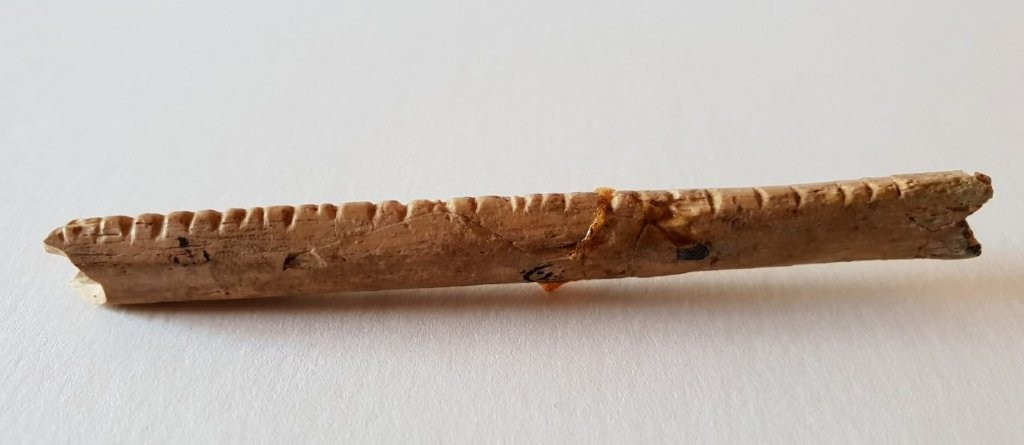
\includegraphics[width=0.45\textwidth]{bilder/lebombo-bone.png}
	\hfill
	\includegraphics[width=0.45\textwidth]{bilder/ishango_bone.jpg}
	\caption{Links: Lebombo-Knochenstück (ca.\ 35.000 Jahre alt, Südafrika). 
		Rechts: Ishango-Knochen (ca.\ 20.000 Jahre alt, Zentralafrika). 
		Beide zeigen regelmäßige Einkerbungen, die als frühe Zählhilfen gedeutet werden. 
		Der Ishango-Knochen wird heute im \emph{Königlichen Belgischen Institut für Naturwissenschaften} in Brüssel aufbewahrt.}
	\label{fig:knochen}
\end{figure}

\HistoryBox{Der Ishango-Knochen}{box:ishango}{%
	Der \emph{Ishango-Knochen} wurde 1960 von 
	Jean de Heinzelin de Braucourt in Zentralafrika entdeckt und ist etwa 20.000 Jahre alt. 
	
	Auf dem Knochen finden sich drei Spalten von Einkerbungen, 
	die nicht zufällig verteilt sind, sondern in Gruppen geordnet erscheinen. 
	Wahrscheinlich diente er als eine Art \emph{Zählstab}\index{Zählstab} – 
	möglicherweise zur Beobachtung des \emph{Mondzyklus}\index{Mondzyklus} 
	oder zur Zählung von Vorräten.
	
	Besonders auffällig: Einige Gruppierungen entsprechen \emph{Primzahlen}\index{Primzahlen} 
	(11, 13, 17, 19). Ob dies Zufall oder Absicht war, bleibt offen. 
	Der Knochen zeigt jedoch, dass Menschen schon in der Altsteinzeit 
	Zahlen nutzten, um Muster in ihrer Welt zu erkennen und festzuhalten.
}

Auch andernorts nutzten Menschen Einkerbungen, Knoten oder Steine als einfache Zählhilfen. 
Kerbhölzer dienten über Jahrtausende zur Aufzeichnung von Vorräten, Abgaben oder Schulden – 
bis in die Neuzeit hinein, etwa im Alpenraum. 
Überall griff man unabhängig zur gleichen Idee: 
Einkerbungen als elementare Zählhilfe.

\subsubsection*{Vom Zählen zum Zahlbegriff}
\phantomsection
Neben archäologischen Funden zeigt auch die \emph{Sprachforschung}\index{Sprachforschung}, 
dass Menschen ihre Umwelt zunächst nur grob in kleine und große Mengen unterteilten – 
anfangs: \emph{eins}, \emph{zwei}, \emph{viele}. 

Manche traditionellen Kulturen kennen bis heute nur sehr wenige \emph{Zahlwörter}\index{Zahlen}, 
oft lediglich die Unterscheidung \glqq eins\grqq, \glqq zwei\grqq{} und \glqq viele\grqq, 
etwa in \emph{Papua-Neuguinea}\index{Papua-Neuguinea} oder \emph{Australien}\index{Australien}. 

Das zeigt: \emph{Zahlen}\index{Zahlen} sind keine Selbstverständlichkeit, 
sondern eine kulturelle \emph{Erfindung}, entstanden aus praktischen Bedürfnissen 
wie \emph{Handel}\index{Handel}, \emph{Vorratshaltung}\index{Vorratshaltung} 
oder \emph{Kalenderrechnung}\index{Kalenderrechnung}. 

Überall – in Afrika, Asien, Europa oder Ozeanien – entwickelten Menschen Zählhilfen 
und \emph{Zahlbegriffe}\index{Zahlbegriff}. 
Das Bedürfnis, die Welt in Zahlen zu fassen, spiegelt eine tiefe Struktur der 
\emph{Wirklichkeit}\index{Wirklichkeit} wider.



% =====================================================
% 2.2 Irrationale Zahlen – die Krise der Griechen
% =====================================================

\subsection{Irrationale Zahlen – die Krise der Griechen}
\label{sec:2.2_irrat}

\subsubsection*{Ausgangspunkt: Pythagoras und die Pythagoreer}
\phantomsection
Die frühen griechischen Mathematiker\index{Griechen}, vor allem die Schule der 
\emph{Pythagoreer}\index{Pythagoreer}, waren überzeugt, dass sich die Welt vollständig 
durch \emph{ganze Zahlen}\index{ganze Zahlen} und \emph{Brüche}\index{Brüche} beschreiben lässt. 
Ihr Leitsatz lautete: „Alles ist Zahl.“ 
Der \emph{Satz des Pythagoras}\index{Satz des Pythagoras} war dafür das zentrale Symbol.

\subsubsection*{Erste Erkenntnisse: Inkommensurabilität}
\phantomsection
Beim Quadrat mit Seitenlänge $1$ wollten die Pythagoreer die Länge der Diagonale berechnen. 
Nach dem Satz des Pythagoras gilt:
\[
c^2 = 1^2 + 1^2 = 2 \quad \Rightarrow \quad c = \sqrt{2}.
\]

Die Zahl $\sqrt{2}$ ließ sich jedoch durch keinen Bruch zweier ganzer Zahlen darstellen. 
Damit war klar: Es gibt \emph{inkommensurable Längen}\index{inkommensurabel}, 
die kein gemeinsames Maß besitzen. 
Die Seitenlänge $1$ und die Diagonale $\sqrt{2}$ sind inkommensurabel.
Diese Erkenntnis stellte die Grundüberzeugung der Pythagoreer in Frage, 
dass die Welt ausschließlich durch ganze Zahlen und Brüche erklärbar sei.

\subsubsection*{Die Krise der Griechen}
\phantomsection
Die Entdeckung der Irrationalität stürzte die Pythagoreer in eine intellektuelle Krise.  
Der Überlieferung nach soll \emph{Hippasos von Metapont}\index{Hippasos von Metapont} 
diese Tatsache erkannt haben – 
die Legende berichtet sogar, dass er von seinen Brüdern ertränkt wurde, 
weil er dieses „Geheimnis“ preisgab. 
Ob die Geschichte wahr ist oder nicht: 
Sicher ist, dass die Entdeckung der Irrationalität 
die griechische Mathematik tief erschütterte. 

\subsubsection*{Der Beweis}
\phantomsection
Einen strengen Beweis für die Irrationalität formulierte \emph{Euklid}\index{Euklid} 
im 10.~Buch seiner \emph{Elemente}\index{Elemente (Euklid)}. 
Er basiert auf einem klassischen Widerspruchsargument:

\MatheBox{Widerspruchsbeweis für $\sqrt{2}$}{box:beweis_wurzel2}{%
	Angenommen, $\sqrt{2}$ sei rational, also $\sqrt{2}=\tfrac{p}{q}$ mit 
	ganzen Zahlen $p,q$, die teilerfremd sind. 
	Dann gilt $2q^2=p^2$. 
	Daraus folgt: $p^2$ ist gerade, also ist auch $p$ gerade. 
	Schreiben wir $p=2r$, dann gilt $2q^2=(2r)^2=4r^2$, also $q^2=2r^2$. 
	Damit ist auch $q$ gerade. 
	
	Somit sind $p$ und $q$ beide gerade, also nicht teilerfremd. 
	Dies widerspricht der Annahme. 
	Damit ist $\sqrt{2}$ irrational.
}

Anschaulich bedeutet dies: 
Es gibt kein gemeinsames Maß, 
mit dem man gleichzeitig die Seitenlänge $1$ und die Diagonale $\sqrt{2}$ 
genau abmessen könnte. 
Jeder Bruch führt irgendwann in einen Widerspruch. 
$\sqrt{2}$ gehört also nicht zur Welt der Brüche, 
sondern eröffnet die neue Zahlenwelt der \emph{irrationalen Zahlen}\index{irrationale Zahlen}.
Die ausführliche Herleitung des Beweises findet sich in 
Anhang~\ref{anhangA_wurzel2}.

\subsubsection*{Näherungen und Berechnung}
\phantomsection
Trotz der Irrationalität blieb $\sqrt{2}$ unverzichtbar. 
Darum entwickelten verschiedene Kulturen Verfahren, den Wert möglichst genau zu bestimmen.

\paragraph{Indische Näherung (Śulba-Sūtras).}
In den altindischen \emph{Śulba\-/Sūtras}\index{Śulba-Sūtras}\index{Indien!Mathematik}
findet sich eine berühmte Näherungsregel für $\sqrt{2}$:
\[
\sqrt{2}\approx 1+\frac{1}{3}+\frac{1}{3\cdot 4}\;-\;\frac{1}{3\cdot 4\cdot 34}
\;=\;1.414\,215\ldots
\]
Schon sechs Nachkommastellen stimmen mit dem exakten Wert überein.

\paragraph{Griechische Verfahren: Iteration und Kettenbruch.}
Arithmetisch nutzten die Griechen das Verfahren 
$x_{n+1}=\tfrac{1}{2}(x_n+\tfrac{2}{x_n})$, 
das rasch zu $\sqrt{2}$ konvergiert – 
heute bekannt als \emph{Newton-Verfahren}.  
Geometrisch wurde die sogenannte \emph{Anthyphairesis} verwendet, 
eine frühe Form des Kettenbruchs:
\[
\sqrt{2}=[1;\overline{2}]=1+\cfrac{1}{2+\cfrac{1}{2+\cdots}}
\]
Die Konvergenten ($3/2,\ 7/5,\ 17/12,\dots$) liefern immer bessere Bruchnäherungen; 
das periodische Muster $\overline{2}$ macht die Irrationalität sichtbar.

\HinweisBox{Mathematik als Entdeckung}{box:mathematik_entdeckung}{%
	Die Entdeckung der irrationalen Zahlen war ein Wendepunkt: 
	Zahlen sind keine bloßen Erfindungen, sondern beschreiben Strukturen, 
	die in der Natur tatsächlich vorkommen. 
	Das Quadrat mit Seitenlänge $1$ „erzwingt“ die Existenz von $\sqrt{2}$.
}

% =====================================================
% 2.3 Null und negative Zahlen
% =====================================================

\subsection{Null und negative Zahlen}
\label{sec:2.3_null_negative}

\subsubsection*{Einleitung}
\phantomsection
Die Vorstellung von \emph{Nichts}\index{Nichts} als Zahl und die Idee von \emph{negativen Zahlen}\index{negative Zahlen} 
sind für uns heute selbstverständlich. 
Historisch jedoch war ihre Entwicklung lang und von Widerständen begleitet. 
Für viele Kulturen war es kaum vorstellbar, 
dass es eine Zahl für „nichts“ geben sollte – oder gar für „weniger als nichts“. 

\subsubsection*{Die Null – Zahl aus dem Nichts}
\phantomsection
Schon die Babylonier nutzten ein Platzhaltersymbol, wenn eine Stelle leer blieb. 
Eine wirkliche \emph{Null als Zahl} entwickelte sich jedoch erst in Indien.  
Dort formulierte \textbf{Brahmagupta}\index{Brahmagupta} im Jahr 628 n.\,Chr. erstmals Rechenregeln mit $0$ 
(in seinem \emph{Brahmasphutasiddhanta}).  
Über die arabische Welt gelangte das Konzept nach Europa und wurde 
durch \textbf{Leonardo Fibonacci}\index{Fibonacci, Leonardo} in seinem \emph{Liber Abaci} (1202) verbreitet.

Viele Philosophen und Theologen taten sich mit der Null schwer. 
Wie konnte „Nichts“ eine Zahl sein? 
In Europa galt sie lange als verdächtig oder sogar gefährlich, 
da sie mit der Idee des Abgrunds oder des Nichtseins verbunden war.  
Heute ist die Null Grundlage des Stellenwertsystems und 
unverzichtbar für die moderne Mathematik.

\subsubsection*{Negative Zahlen – Schulden und Temperaturen}
\phantomsection
Negative Zahlen tauchten bereits in China um 200 v.\,Chr. auf, 
in den \emph{Neun Büchern über die Mathematik}\index{China!Neun Bücher über die Mathematik}.  
Man unterschied positive und negative Werte mit verschiedenfarbigen Rechenstäbchen: 
rot für Gewinne, schwarz für Verluste.  
Auch in Indien wurden negative Zahlen verwendet, etwa zur Darstellung von Schulden oder Defiziten. 

\begin{figure}[ht]
	\centering
	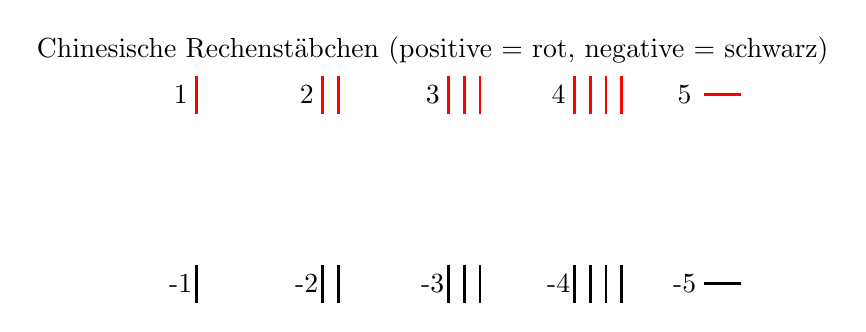
\begin{tikzpicture}[scale=0.8, line width=1pt]
		\node at (4,3.2) {Chinesische Rechenstäbchen (positive = rot, negative = schwarz)};
		% Positive Zahlen (rot)
		\foreach \n/\count in {1/1, 2/2, 3/3, 4/4} {
			\node at (2*\n-2,2.5) {\n};
			\foreach \i in {1,...,\count} {
				\draw[red] (2*\n-2+0.25*\i,2.2) -- (2*\n-2+0.25*\i,2.8);
			}
		}
		\node at (8,2.5) {5};
		\draw[red] (8.3,2.5) -- (8.9,2.5);
		% Negative Zahlen (schwarz)
		\foreach \n/\count in {1/1, 2/2, 3/3, 4/4} {
			\node at (2*\n-2,-0.5) {-\n};
			\foreach \i in {1,...,\count} {
				\draw[black] (2*\n-2+0.25*\i,-0.8) -- (2*\n-2+0.25*\i,-0.2);
			}
		}
		\node at (8,-0.5) {-5};
		\draw[black] (8.3,-0.5) -- (8.9,-0.5);
	\end{tikzpicture}
	\caption{Chinesische Rechenstäbchen: positive Zahlen (rot), negative Zahlen (schwarz).}
	\label{fig:rod_numerals_colored}
\end{figure}

\MatheBox{Rechenregeln für negative Zahlen}{box:regeln_negative}{%
	Heute sind die Regeln vertraut:
	\[
	(+a)+(-b)=a-b, \quad (-a)+(-b)=-(a+b),
	\]
	\[
	(-a)\cdot(-b)=+ab, \quad (-a)\cdot b=-(ab).
	\]
	Doch diese einfachen Regeln wurden in Europa erst sehr spät akzeptiert. 
	\textbf{René Descartes}\index{Descartes, René} bezeichnete negative Zahlen noch als 
	„falsche Zahlen“.
}

Viele Mathematiker fragten sich: 
Wie kann man „weniger als nichts“ besitzen? 
Ein negatives Ergebnis schien absurd. 
Erst durch praktische Anwendungen wie Buchhaltung (Schulden) oder 
Temperaturmessungen unter Null wurde ihre Nützlichkeit offensichtlich.
Mit der Null und den negativen Zahlen erweiterte sich das Zahlensystem entscheidend: 
Mathematik begann, nicht nur das Zählen von Dingen zu beschreiben, 
sondern auch Abwesenheit und Gegensätze. 
So entstand die moderne Zahlengerade, 
auf der sich alle ganzen Zahlen von $-\infty$ bis $+\infty$ anordnen lassen.

% =====================================================
% 2.4 Komplexe Zahlen – eine unerwartete Erweiterung
% =====================================================

\subsection{Komplexe Zahlen – eine unerwartete Erweiterung}
\label{sec:2.4_komplexe}

\subsubsection*{Einleitung}
\phantomsection
Während Brüche, irrationale Zahlen, die Null und die negativen Zahlen jeweils aus praktischen 
Problemen hervorgegangen sind, entstand die nächste Erweiterung des Zahlbegriffs fast beiläufig: 
die sogenannten \emph{komplexen Zahlen}.  
Sie tauchten auf, als man versuchte, Gleichungen zu lösen, 
die mit den bekannten Zahlenarten nicht lösbar waren.

\subsubsection*{Erste Ansätze in der Renaissance}
\phantomsection
Im 16.~Jahrhundert beschäftigten sich italienische Mathematiker wie 
\textbf{Scipione del Ferro}\index{del Ferro, Scipione}, 
\textbf{Niccolò Tartaglia}\index{Tartaglia, Niccolò} und 
\textbf{Gerolamo Cardano}\index{Cardano, Gerolamo} mit kubischen Gleichungen.  
Bei manchen Lösungswegen traten Zwischenschritte mit $\sqrt{-1}$ auf – 
obwohl das Endergebnis wieder eine reelle Zahl war.  
Cardano nannte diese Ausdrücke „sophistische Wurzeln“ – 
er schrieb sie zwar auf, verstand sie aber nicht.  
Man hielt sie für eine Art Rechenkuriosität: notwendig im Lösungsweg, 
aber ohne eigenständige Bedeutung.

\subsubsection*{Bombelli und die Wende}
\phantomsection
Der italienische Mathematiker \textbf{Rafael (Raffaele) Bombelli}\index{Bombelli, Rafael} erkannte um 1572, 
dass man mit diesen „imaginären Zahlen“ konsistent rechnen kann, 
wenn man sie wie gewöhnliche Zahlen behandelt und $i^2=-1$ setzt.  
Damit legte er den Grundstein für die Theorie der komplexen Zahlen.

Noch lange galten komplexe Zahlen als „fiktiv“ oder „imaginär“.  
Erst im 18.~und 19.~Jahrhundert, bei \textbf{Leonhard Euler}\index{Euler, Leonhard}, 
\textbf{Carl Friedrich Gauss}\index{Gauss, Carl Friedrich} und 
\textbf{Jean-Robert Argand}\index{Argand, Jean-Robert}, 
setzte sich die Erkenntnis durch:  
Komplexe Zahlen sind nicht nur Hilfsmittel, sondern eine 
notwendige und vollwertige Erweiterung des Zahlbegriffs.  

\subsubsection*{Bedeutung}
\phantomsection
Heute bilden die komplexen Zahlen ein Fundament der modernen Mathematik.  
Sie garantieren mit dem \emph{Fundamentalsatz der Algebra}\index{Fundamentalsatz der Algebra}, 
dass jedes Polynom eine Lösung besitzt, 
und sind in Physik und Technik unverzichtbar – etwa für Schwingungen, Wellen, 
Quantenmechanik und Elektrotechnik.

Die ausführliche historische Herleitung und die formale Einführung von $i^2=-1$ 
finden sich im Anhang~\ref{anhangA_i}.

% =====================================================
% 2.5 Fazit
% =====================================================

\subsection{Fazit: Zahlen als entdeckte Struktur}

Vom Zählen der Herden bis zur Einführung der komplexen Zahlen zeigt sich ein roter Faden: 
Neue Zahlenarten entstehen nicht willkürlich, sondern immer dann, wenn die bisherigen 
Zahlen nicht mehr ausreichen.  

\begin{itemize}
	\item Die \emph{natürlichen Zahlen}\index{natürliche Zahlen} entstanden aus dem praktischen Bedürfnis zu zählen.  
	\item \emph{Irrationale Zahlen}\index{irrationale Zahlen} wurden entdeckt, als die Geometrie den Bereich der Brüche sprengte.  
	\item Die \emph{Null}\index{Null} und die \emph{negativen Zahlen}\index{negative Zahlen} öffneten den Blick für Abwesenheit und Gegensätze.  
	\item Die \emph{komplexen Zahlen}\index{komplexe Zahlen} machten scheinbar unlösbare Gleichungen lösbar und führten zur Vollständigkeit der Mathematik.  
\end{itemize}

\HinweisBox{Zahlen als universelle Struktur}{box:mathematik_entdeckung_fazit}{%
	Zahlen sind keine freie Erfindung des Menschen.  
	Sie wurden Schritt für Schritt \emph{entdeckt}, weil die Welt selbst 
	eine innere Struktur hat, die wir in Zahlen fassen können.  
	Durch logisches Weiterdenken und konsequentes Rechnen erschlossen sich immer neue Zahlbereiche – 
	von den Kerben auf Knochen bis hin zur komplexen Ebene.  
}

	
\chapter{Algebra und Gleichungen}
\label{chap:III_algebra}
\label{chap:III_qubit}
\setcounter{section}{3}
\setcounter{subsection}{0}
\setcounter{subsubsection}{1}
\setcounter{secnumdepth}{3}
\subsection{Die arabische Mathematik und die Geburt der Algebra}
\label{sec:3.1_arabische_mathematik}

Nach den Griechen, Indern und Babyloniern war es die arabisch-islamische Welt, 
die die Mathematik auf eine neue, systematische Ebene hob. 
Während in Europa das antike Wissen weitgehend verloren ging, 
bewahrten und erweiterten Gelehrte wie 
\emph{al-Chwarizmi}\index{al-Chwarizmi, Muhammad ibn Musa}, 
\emph{Omar Chayyām}\index{Chayyām, Omar} und 
\emph{al-Karaji}\index{al-Karaji, Abu Bakr} die Erkenntnisse ihrer Vorgänger. 

Im 9.~Jahrhundert verfasste \emph{al-Chwarizmi} in Bagdad das Werk 
\emph{„Kitāb al-jabr wa’l-muqābala“}\index{Kitāb al-jabr wa’l-muqābala}, 
das als Geburtsstunde der \emph{Algebra}\index{Algebra} gilt. 
Der Begriff „al-jabr“ bedeutet sinngemäß „das Wiederherstellen“ oder „das Ergänzen“, 
„al-muqabala“ bezeichnet „das Gegenüberstellen“. 
Gemeint war damit eine Methode, Unbekanntes zu isolieren und Gleichungen zu vereinfachen – 
eine Revolution im Denken über Zahlen und Formen. 

\HistoryBox{Von der Praxis zur Theorie}{hist:algebra_praxis}{
	Im Mittelpunkt der arabischen Mathematik stand anfangs die Lösung praktischer Probleme: 
	Verteilung von Erbschaften, Berechnung von Grundstücksflächen, 
	Bestimmung von Handelsanteilen oder astronomische Messungen. 
	Doch aus diesen konkreten Aufgaben entwickelte sich ein allgemeines Verfahren, 
	Unbekannte zu bestimmen – die Geburt der symbolischen Methode.
}

Ein klassisches Beispiel aus der frühen arabischen Mathematik ist die Berechnung von Erbanteilen. 
Nach islamischem Recht erhält eine Frau den achten Teil des Nachlasses, 
der Rest wird unter den Söhnen gleich verteilt. 
Beträgt das Erbe insgesamt 600~Dinar, so ergibt sich:

\[
1 = \tfrac{1}{8} + 2x,
\]
wobei \(x\) den Anteil eines Sohnes beschreibt. 
Nach Umformen folgt \(x = \tfrac{7}{16}\). 
Damit erhält jeder Sohn \(x \cdot 600 = 262{,}5\)~Dinar, 
die Frau \(75\)~Dinar.

\DidaktikBox{Vom praktischen Problem zur abstrakten Gleichung}{did:algebraischer_denken}{
	Die arabischen Mathematiker formulierten solche Beziehungen symbolisch 
	und lösten sie durch \emph{al-jabr} (Ergänzen) und \emph{al-muqabala} (Gegenüberstellen). 
	So entstand aus einem alltäglichen Rechenproblem die Idee der allgemeinen Gleichung – 
	der Beginn der Algebra als abstraktes Denken.
}

\HinweisBox{Ein gemeinsames Erbe}{hinweis:algebra_herkunft}{
	Die arabischen Mathematiker erfanden die Algebra nicht aus dem Nichts. 
	Sie knüpften an das Wissen der Babylonier, Griechen und Inder an. 
	Schon die Babylonier lösten Gleichungen der Form \(x^2 + bx = c\) 
	mit tabellarischen Methoden, und die Griechen beschrieben geometrische Zusammenhänge, 
	die im Kern algebraisch waren. 
	In Indien entstanden symbolische Rechenverfahren für Unbekannte (\emph{yāvattavat}). 
	Die arabischen Gelehrten verbanden all diese Traditionen, 
	gaben ihnen eine einheitliche Sprache und machten daraus ein geschlossenes System – 
	die \emph{Al-jabr}, die wir heute Algebra nennen.
}

Ein bekanntes Beispiel aus Al-Chwarizmis Werk lautet:
\begin{quote}
	„Ein Quadrat und zehn seiner Wurzeln ergeben neununddreißig.“
\end{quote}
Heute würden wir dies als
\[
x^2 + 10x = 39
\]
schreiben.  
Al-Chwarizmi dachte jedoch geometrisch: Das Glied \(x^2\) stellte ein Quadrat dar, 
dessen Seitenlänge \(x\) ist. Die Terme \(10x\) bildeten zwei Rechtecke der Breite~5, 
die an zwei Seiten des Quadrats anliegen.  
Das fehlende kleine Quadrat in der Ecke, das die Figur zu einem größeren Quadrat ergänzt, 
hat die Fläche \(5^2 = 25\).  
Durch Hinzufügen dieser Fläche wird das Gebilde zu einem vollständigen Quadrat:
\[
x^2 + 10x + 25 = 39 + 25,
\]
also \((x+5)^2 = 64\), woraus \(x = 3\) folgt.
\subsubsection*{Graphische Darstellung der quadratischen Ergänzung}
\phantomsection
\begin{figure}[h!]
	\centering
	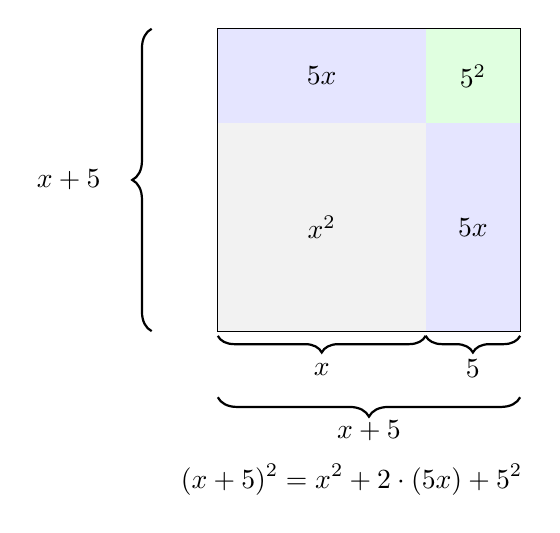
\begin{tikzpicture}[scale=0.12, thick]
		\def\xlen{22}   % Länge x (grafisch)
		\def\five{10}   % Länge 5  (grafisch)
		
		% Gesamtquadrat (x+5)
		\draw (0,0) rectangle (\xlen+\five,\xlen+\five);
		
		% Unterteilung
		\draw (\xlen,0) -- (\xlen,\xlen+\five);
		\draw (0,\xlen) -- (\xlen+\five,\xlen);
		
		% Füllungen
		\fill[gray!10] (0,0) rectangle (\xlen,\xlen);                 % x^2
		\fill[blue!10] (0,\xlen) rectangle (\xlen,\xlen+\five);       % 5x (oben)
		\fill[blue!10] (\xlen,0) rectangle (\xlen+\five,\xlen);       % 5x (rechts)
		\fill[green!12] (\xlen,\xlen) rectangle (\xlen+\five,\xlen+\five); % 5^2
		
		% Beschriftungen
		\node at ({\xlen/2},{\xlen/2}) {$x^2$};
		\node at ({\xlen/2},{\xlen+\five/2}) {$5x$};
		\node at ({\xlen+\five/2},{\xlen/2}) {$5x$};
		\node at ({\xlen+\five/2},{\xlen+\five/2}) {$5^2$};
		
		% Nur eine geschweifte Klammer unten (5 dann x)
	%	\draw [decorate, decoration={brace, amplitude=6pt}]
	%	(0,-2) -- (\five,-2) node[midway, yshift=-10pt] {$5$};
		\draw [decorate, decoration={brace, amplitude=6pt,mirror}]
		(0,-0.5) -- (\xlen,-0.5) node[midway, yshift=-12pt] {$x$};
			\draw [decorate, decoration={brace, amplitude=6pt,mirror}]
		(\xlen,-0.5) -- (\xlen+10,-0.5) node[midway, yshift=-12pt] {$5$};
		% Gesamtlänge unten (x+5)
		\draw [decorate, decoration={brace, amplitude=7pt,mirror}]
		(0,-7) -- (\xlen+\five,-7) node[midway, yshift=-12pt] {$x+5$};
		
		% Linke Gesamtlänge (optional, schmal)
		\draw [decorate, decoration={brace, amplitude=7pt}]
		(-7,0) -- (-7,\xlen+\five) node[midway, xshift=-30pt] {$x+5$};
		
		% Titel
		\node[below right] at (-5,\xlen+\five-45)
		{$\displaystyle (x+5)^2 = x^2 + 2\cdot(5x) + 5^2$};
	\end{tikzpicture}
	\caption{Aus den Teilflächen $x^2$, $5x$ und $5^2$ entsteht das Quadrat $(x+5)^2$.}
\end{figure}





Diese geometrische Methode des Ergänzens – das eigentliche „al-jabr“ – 
führte direkt zur allgemeinen Regel für quadratische Gleichungen, 
die wir heute in symbolischer Form schreiben.  

\DidaktikBox{Der Ursprung des Wortes „Algorithmus“}{did:algorithmus}{
	Der Name \emph{al-Chwarizmi} wurde im Lateinischen zu „Algoritmi“ verfremdet. 
	Daraus entstand das Wort \emph{Algorithmus}\index{Algorithmus}. 
	Damit geht auch ein zweiter Grundpfeiler der modernen Mathematik 
	– die systematische, regelhafte Berechnung – 
	auf die arabische Wissenschaft zurück.
}

Die Algebra war also weniger eine Entdeckung im modernen Sinn, 
sondern eine geistige Neuordnung des vorhandenen Wissens. 
Sie verband die indischen Zahlensysteme mit griechischer Geometrie 
und formte daraus ein allgemeines Rechenverfahren. 
Damit begann die Mathematik, ihre eigene Sprache zu entwickeln – 
eine Sprache der Symbole, Regeln und Abstraktionen.

\subsection{Gleichungen als Werkzeuge zur Problemlösung}
Gleichungen wurden zum universellen Werkzeug, um unbekannte Größen zu berechnen. 
Von einfachen linearen Gleichungen bis zu quadratischen Formen zeigte sich ihre enorme Nützlichkeit. 

\subsection{Die Entstehung der komplexen Zahlen}
Bei der Lösung höherer Gleichungen traten scheinbar „unmögliche“ Zahlen auf. 
Aus dieser Notwendigkeit heraus entstanden die komplexen Zahlen, die bald eine tiefe Bedeutung erhielten. 

\subsection{Mathematik als System von Regeln}
Mit Algebra und Gleichungen begann die Mathematik, sich stärker als ein in sich geschlossenes Regelwerk zu verstehen. 
Diese Sichtweise prägte die weitere Entwicklung bis in die Moderne. 

	\chapter{Mathematik als Sprache der Natur}
\label{chap:IV_sprache}
\label{chap:IV_algorithmen}
\setcounter{section}{4}
\setcounter{subsection}{0}
\setcounter{subsubsection}{1}
\setcounter{secnumdepth}{3}
\setlength{\parindent}{0pt}


\subsection{Galilei und die neue Physik}
\textbf{Galilei}\index{Galilei, Galileo} erkannte, dass die Naturgesetze mathematisch formulierbar sind. 
Seine Experimente mit fallenden Körpern machten deutlich: Bewegung folgt klaren Regeln, die sich in Gleichungen ausdrücken lassen. 

\subsection{Funktionen und Bewegungsgesetze}
Mit dem Begriff der \textbf{Funktion}\index{Funktion} konnten Zusammenhänge präzise beschrieben werden. 
Ob Geschwindigkeit, Kraft oder Energie – in jedem Fall wurde eine mathematische Form die Sprache der Natur. 

\subsection{Differentialgleichungen und Wachstum}
Die Einführung der \textbf{Differentialgleichungen}\index{Differentialgleichung} eröffnete neue Möglichkeiten. 
Von der Mechanik über die Himmelskörper bis hin zu Wachstumsprozessen ließen sich Entwicklungen nun systematisch erfassen. 

\subsection{Von der Mechanik zur modernen Physik}
Die Sprache der Mathematik blieb nicht auf die klassische Mechanik beschränkt. 
Auch Elektrodynamik, Relativitätstheorie und Quantenphysik beruhen auf denselben Prinzipien – 
die Natur spricht überall dieselbe Sprache. 

	\chapter{Wahrscheinlichkeiten und Zufall}
\label{chap:V_wahrscheinlichkeit}
\label{chap:V_realisationen}
\setcounter{section}{5}
\setcounter{subsection}{0}
\setcounter{subsubsection}{1}
\setcounter{secnumdepth}{3}
\setlength{\parindent}{0pt}


\subsection{Würfel und die Entstehung der Wahrscheinlichkeitstheorie}
Das Spiel mit Würfeln war mehr als Unterhaltung – es führte zur Frage, 
wie man den Zufall mathematisch beschreiben kann. 
Hier entstand die Wahrscheinlichkeitstheorie als eigenständiges Gebiet. 

\subsection{Statistik und Naturgesetze}
Mit der Statistik lernte man, viele Einzelereignisse zu ordnen und zu mitteln. 
So konnten Naturgesetze sichtbar werden, die sich nur in großen Zahlen offenbaren. 

\subsection{Quantenmechanik und Zufall}
In der Quantenmechanik ist der Zufall nicht nur ein Mangel an Wissen, 
sondern ein grundlegendes Prinzip der Natur. 
Die Mathematik der Wahrscheinlichkeiten ist hier Teil der Wirklichkeit selbst. 

\subsection{Ordnung im Chaos}
Selbst in scheinbar chaotischen Prozessen zeigen sich Strukturen. 
Die moderne Mathematik des Chaos und der nichtlinearen Systeme 
macht deutlich, dass Zufall und Ordnung eng verbunden sind. 

	\chapter{Abstraktion und Struktur}
\label{chap:VI_abstraktion}

\setcounter{section}{6}
\setcounter{subsection}{0}
\setcounter{subsubsection}{1}
\setcounter{secnumdepth}{3}


\subsection{Vektoren und Räume}
Mit der Einführung von \textbf{Vektoren}\index{Vektoren} und abstrakten \textbf{Räumen}\index{Räume} 
konnte man geometrische und physikalische Probleme auf eine neue Ebene heben. 
Damit begann die Mathematik, Strukturen unabhängig von Anschauung zu betrachten. 

\subsection{Symmetrien und Invarianz}
\textbf{Symmetrien}\index{Symmetrien} spielen in Mathematik und Physik eine fundamentale Rolle. 
Sie zeigen, welche Eigenschaften eines Systems sich nicht ändern – auch wenn sich die Darstellung wandelt. 

\subsection{Mathematik als universelles Strukturprinzip}
Immer deutlicher wurde, dass Mathematik nicht nur Werkzeuge liefert, 
sondern selbst die Form der Naturgesetze bestimmt. 
Abstrakte Prinzipien wie Invarianz oder Transformationen prägen unser Verständnis der Welt. 

\subsection{Abstraktion als Weg zur Wirklichkeit}
Was wie reine Gedankenarbeit wirkt, erweist sich oft als Beschreibung realer Phänomene. 
Abstraktion ist damit kein Gegensatz zur Realität, 
sondern ein Weg, deren Struktur sichtbar zu machen. 

	git\chapter{Mathematik und Philosophie}
\label{chap:VII_philosophie}
\label{chap:VII_anwendungen}
\setcounter{section}{7}
\setcounter{subsection}{0}
\setcounter{subsubsection}{1}
\setcounter{secnumdepth}{3}
% Boxen-Stile definieren




% ================================
% Teil III – Mathematik und Philosophie
% ================================



\subsection{Platon und die Ideenwelt}
Für Platon war Mathematik ein Teil der ewigen Ideenwelt. 
Zahlen und geometrische Formen existierten unabhängig vom Menschen. 

\subsection{Aristoteles und die praktische Mathematik}
Aristoteles betonte den praktischen Nutzen der Mathematik – 
als Werkzeug für Logik, Physik und Naturbeschreibung. 

\subsection{Kant und die Bedingungen der Erkenntnis}
Kant sah in der Mathematik eine apriorische Form unseres Denkens: 
Raum und Zeit sind die Grundlage, auf der wir Naturgesetze erkennen können. 

\subsection{Moderne Positionen}
Heute wird die Frage neu gestellt: 
Ist Mathematik eine menschliche Erfindung, ein nützliches Sprachspiel – 
oder eine Entdeckung von Strukturen, die unabhängig von uns existieren? 
Philosophie und Naturwissenschaft bleiben hier eng verbunden. 

	
\chapter{Mathematik im 21. Jahrhundert}
\label{chap:VIII_21jh}
\label{chap:VII_philosophie}
\label{chap:VIII_ausblick}
\setcounter{section}{8}
\setcounter{subsection}{0}
\setcounter{subsubsection}{1}
\setcounter{secnumdepth}{3}
% ================================
% Teil IV – Mathematik im 21. Jahrhundert
% ================================



\subsection{Gödel und die Grenzen formaler Systeme}
Mit seinen Unvollständigkeitssätzen zeigte \textbf{Gödel, Kurt}\index{Gödel, Kurt}, 
dass es in jedem formalen System wahre Aussagen gibt, die nicht beweisbar sind. 
Dies veränderte das Verständnis von Mathematik grundlegend. 

\subsection{Computer und künstliche Intelligenz}
Computer haben die Mathematik praktisch und theoretisch revolutioniert. 
Von automatisierten Beweisen bis hin zu \textbf{künstlicher Intelligenz}\index{Künstliche Intelligenz} 
stellt sich die Frage: Lösen Maschinen nur Aufgaben – oder entdecken sie selbst Strukturen? 

\subsection{Mathematik und moderne Physik}
Die heutige Physik – von der Relativitätstheorie bis zur Quantenfeldtheorie – 
zeigt, dass Mathematik nicht nur Werkzeug ist, sondern den Rahmen der Naturgesetze vorgibt. 

\subsection{Ausblick: Die Struktur der Welt}
Die Reise führt zu einer offenen Frage: 
Ist Mathematik die Sprache, die wir erfinden – oder die Struktur, die wir entdecken? 
Vielleicht ist sie beides zugleich: ein Spiegel des Geistes und der Welt. 

	
	% Anhänge
	%===========================
% Anhang A: Mathematische Grundlagen
%===========================


\appendix
\renewcommand{\thesection}{A.\arabic{section}}

\renewcommand{\thechapter}{A}
\chapter{Mathematische Grundlagen}
\label{anhangA_mathe}



\noindent
Die Kapitel des Hauptteils haben gezeigt, wie sich der Zahlbegriff im Laufe der Geschichte 
erweitert hat – von den natürlichen Zahlen bis zu den komplexen Zahlen. 
Um den Lesefluss nicht zu überfrachten, wurden die mathematischen Details dabei 
meist nur skizziert. 

In diesem Anhang finden sich einige der klassischen Herleitungen, die für das Verständnis 
der Entwicklung des Zahlbegriffs zentral sind. Sie zeigen, wie Logik und Beweisführung 
neue Zahlarten notwendig machten. 


Damit dient dieser Anhang als Ergänzung: Er bietet die mathematische Tiefe für alle, 
die genauer verstehen möchten, wie die neuen Zahlbereiche Schritt für Schritt 
logisch begründet wurden.

\newpage
\refstepcounter{section}\label{anhangA_wurzel2}
\section*{A.1 Widerspruchsbeweis für die Irrationalität von $\sqrt{2}$}
\addcontentsline{toc}{section}{A.1 Widerspruchsbeweis für die Irrationalität von $\sqrt{2}$}
\label{anhangA_wurzel2}

\noindent
% --- A.1 Beweis der Irrationalität von sqrt(2) ---



\subsubsection*{Vorbemerkung (Lemma)}
\phantomsection
\textbf{Lemma.} Ist $p^2$ eine \emph{gerade} Zahl, so ist auch $p$ gerade.

\emph{Begründung.} Wäre $p$ ungerade, dann $p=2k+1$ und damit
$p^2=(2k+1)^2=4k^2+4k+1=2(2k^2+2k)+1$ ungerade — Widerspruch. \hfill$\square$

\vspace{0.5em}

\subsubsection*{Beweis (Widerspruchsbeweis)}
\phantomsection
Angenommen, $\sqrt{2}$ sei \emph{rational}. Dann existieren ganze Zahlen $p,q$ ohne gemeinsamen Teiler
($\gcd(p,q)=1$) mit
\[
\sqrt{2}=\frac{p}{q}.
\]
Quadrieren liefert
\[
2=\frac{p^2}{q^2}\quad\Longrightarrow\quad p^2=2q^2.
\]
Damit ist $p^2$ gerade, also nach dem Lemma auch $p$ gerade. Schreibe $p=2r$.
Dann folgt
\[
p^2=(2r)^2=4r^2=2q^2 \;\Longrightarrow\; q^2=2r^2,
\]
also ist auch $q^2$ gerade und damit $q$ gerade.

Damit sind \emph{beide} Zahlen $p$ und $q$ gerade — sie besitzen also den gemeinsamen Teiler $2$.
Das widerspricht der getroffenen Annahme, dass $p$ und $q$ teilerfremd sind. 
Die Ausgangsannahme war folglich falsch, also ist $\sqrt{2}$ \emph{irrational}. \hfill$\square$

\DidaktikBox{Was hier passiert (Idee des Widerspruchs)}{box:idee_wurzel2_lang}{%
	Wir nehmen an, $\sqrt{2}$ sei \emph{doch} eine Bruchzahl in vollständig gekürzter Form $\frac{p}{q}$.
	Aus der Gleichung $p^2=2q^2$ folgt nacheinander, dass $p$ gerade ist und \emph{deshalb} auch $q$ gerade sein muss.
	Damit wäre $\frac{p}{q}$ aber \emph{nicht} vollständig gekürzt. Genau dieser \glqq Teilerfremdheits-Widerspruch\grqq{}
	zeigt: Die Annahme war unmöglich — also ist $\sqrt{2}$ irrational.
}

\HinweisBox{Alternative Sichtweisen}{box:alternativen_wurzel2}{%
	\textbf{(1) Primfaktorzerlegung:} In der eindeutigen Primfaktorzerlegung besitzt $2$ einen \emph{ungeraden}
	Exponenten, während ein Quadrat stets nur \emph{gerade} Exponenten hat — das passt nicht zusammen.\\[0.3em]
	\textbf{(2) Kettenbruch:} Die Darstellung $\sqrt{2}=[1;\overline{2}]$ ist \emph{periodisch unendlich};
	solche Kettenbrüche entsprechen irrationalen Zahlen.
}

\newpage
\refstepcounter{section}\label{anhangA_i}
\section*{A.2 Von negativen Wurzeln zu $i^2=-1$}
\addcontentsline{toc}{section}{A.2 Von negativen Wurzeln zu $i^2=-1$}
\label{anhangA_i}

\noindent
Im 16.~Jahrhundert stießen italienische Mathematiker bei der Lösung kubischer Gleichungen 
auf Ausdrücke wie $\sqrt{-1}$.  
Zunächst galten diese als „unmöglich“, doch \textbf{Rafael (Raffaele) Bombelli}\index{Bombelli, Rafael} 
zeigte, dass man sie konsistent behandeln kann, wenn man $i^2=-1$ setzt.  

\MatheBox{Definition der imaginären Einheit}{box:anhang_i}{%
	Die imaginäre Einheit $i$ wird definiert durch
	\[
	i^2 = -1.
	\]
	Jede komplexe Zahl lässt sich dann als 
	\[
	z = a + bi \quad \text{mit } a,b \in \mathbb{R}
	\]
	schreiben. 
}

\noindent
Dieser Schritt führte zu einer völlig neuen Zahlenwelt. 
Zunächst misstrauisch betrachtet, wurden komplexe Zahlen später durch 
Euler, Gauss und Argand in der Mathematik fest verankert. 
Heute bilden sie eine unverzichtbare Grundlage vieler Gebiete der Mathematik und Physik.

	\cleardoublepage
%\appendix
\renewcommand{\thechapter}{B}

\renewcommand{\thesection}{\Alph{chapter}.\arabic{section}}



\chapter{Boxenverzeichnis}
\label{anhangB}


%\chapter{Boxenverzeichnis}
\label{chap:boxenverzeichnis}
\thispagestyle{empty}


%\addcontentsline{toc}{chapter}{Anhang B – Boxenverzeichnis}


	\cleardoublepage

\renewcommand{\thesection}{\thechapter.\arabic{section}}
\renewcommand{\thechapter}{C}

\chapter{KI in der Wissenschaft – Werkzeug statt Wahrheit}
\phantomsection
\vspace{1em}
\begin{center}
	\LARGE\textbf{KI in der Wissenschaft – Werkzeug statt Wahrheit}
\end{center}

\subsection*{Motivation}
\phantomsection
Dieses Buch entstand aus dem Wunsch, die Grundlagen und Perspektiven der Quanteninformatik – vom Qubit über Algorithmen bis hin zu technischen Realisierungen – verständlich und fundiert darzustellen. 
Dabei wurde ein Werkzeug eingesetzt, das heute immer mehr Einzug in wissenschaftliches Arbeiten hält: \textbf{künstliche Intelligenz}\index{Künstliche Intelligenz}, konkret das Sprachmodell \textbf{ChatGPT}\index{ChatGPT} von OpenAI.

Doch wie lässt sich KI sinnvoll in der Wissenschaft\index{Wissenschaft} nutzen, ohne dass dabei Verständnis, Präzision oder Verantwortung\index{Verantwortung} verloren gehen? Und wie kann man das offenlegen, ohne die eigene wissenschaftliche Arbeit zu relativieren? Dieser Anhang gibt einen transparenten Einblick in den Entstehungsprozess dieses Buches und plädiert für einen verantwortungsvollen Umgang mit KI als Werkzeug – nicht als Wahrheit.

\subsection*{Was eine KI kann – und was nicht}
\phantomsection
KI-gestützte Sprachmodelle wie ChatGPT sind leistungsfähige Hilfsmittel beim Schreiben und Strukturieren. Sie können:
\begin{itemize}
	\item beim Formulieren erster Entwürfe helfen,
	\item komplexe Sachverhalte sprachlich glätten,
	\item Denkanstöße liefern oder Gliederungen vorschlagen,
	\item stilistische Alternativen aufzeigen.
\end{itemize}

Was sie jedoch \textbf{nicht} können:
\begin{itemize}
	\item \textbf{Verstehen}\index{Verstehen} im wissenschaftlichen Sinn,
	\item \textbf{prüfen}, ob eine mathematische Herleitung korrekt ist,
	\item \textbf{physikalische Konzepte oder Algorithmen durchdringen},
	\item \textbf{Quellen kritisch einordnen oder bewerten}.
\end{itemize}

Daher gilt: Eine KI kann \emph{unterstützen}, aber sie \textbf{kann und darf den wissenschaftlichen Erkenntnisprozess nicht ersetzen}. Wer mit KI arbeitet, muss dennoch selbst denken – und das Ergebnis stets kritisch prüfen.

\subsection*{Wie dieses Buch entstanden ist}
\phantomsection
Die Inhalte dieses Buches – von der Struktur über die physikalischen Erklärungen bis zu den mathematischen und algorithmischen Herleitungen – wurden vom Autor konzipiert, recherchiert und verantwortet. ChatGPT kam in folgenden Bereichen unterstützend zum Einsatz:

\begin{itemize}
	\item beim \textbf{Formulieren einzelner Passagen}, z.\,B. bei Einleitungen, Zusammenfassungen oder didaktischen Abschnitten,
	\item zur \textbf{Stilüberprüfung} technischer und algorithmischer Erklärungen,
	\item zur \textbf{Gliederungsentwicklung} in frühen Arbeitsphasen,
	\item zur Reflexion über \textbf{Verständlichkeit}\index{Verständlichkeit} und Leserführung.
\end{itemize}

Entscheidend ist: \textbf{Alle inhaltlichen Aussagen, Formeln, Algorithmen und Interpretationen wurden vom Autor geprüft, hinterfragt, überarbeitet oder verworfen.} Keine KI war an der inhaltlichen Entwicklung der physikalischen oder informatischen Argumentation beteiligt.

\subsection*{Ethische Fragen und wissenschaftliche Verantwortung}
\phantomsection
Die Nutzung von KI in der Wissenschaft wirft berechtigte Fragen auf:

\begin{itemize}
	\item Wie viel darf automatisiert entstehen, ohne dass Autorschaft\index{Autorschaft} verwässert?
	\item Wie geht man mit potenziellen Fehlern\index{Fehler} um?
	\item Wie transparent muss die Nutzung offengelegt werden?
\end{itemize}

Die Antwort liegt in einem Grundprinzip wissenschaftlicher Arbeit: \textbf{Verantwortung}. Wer KI einsetzt, bleibt verantwortlich für das Ergebnis – unabhängig davon, ob einzelne Formulierungen von einem Modell vorgeschlagen wurden.

In diesem Sinne ist KI keine Autorin, sondern ein Werkzeug. Sie kann Prozesse beschleunigen, aber nicht ersetzen, was Wissenschaft im Kern ausmacht: \textbf{kritisches Denken, sorgfältiges Prüfen, methodisches Arbeiten}.

\subsection*{Empfehlungen für den Einsatz in der Forschung}
\phantomsection
Für Wissenschaftler:innen, Lehrende und Studierende ergibt sich daraus ein konstruktiver Weg:

\begin{itemize}
	\item Nutze KI \textbf{bewusst und gezielt} – für sprachliche Unterstützung, nicht für Argumentation, Beweisführung oder Algorithmusentwicklung.
	\item \textbf{Prüfe jede Aussage selbst} – gerade bei komplexen Sachverhalten.
	\item \textbf{Deklariere die Nutzung offen}, wenn es relevant ist – z.\,B. in Vorworten, Anhängen oder Einreichungserklärungen.
	\item Nutze KI nicht zur \textbf{Täuschung}\index{Täuschung} oder zum Feigenblatt, sondern als Hilfe zur besseren Darstellung deiner eigenen Gedanken.
\end{itemize}

\subsection*{Fazit: KI als Werkzeug – aber der Mensch bleibt denkend verantwortlich}
\phantomsection
Künstliche Intelligenz ist weder Ersatz noch Gegner menschlicher Erkenntnis. Sie ist ein \textbf{Werkzeug}\index{Werkzeug}, das bei der wissenschaftlichen Kommunikation helfen kann – \textbf{wenn es bewusst, reflektiert und verantwortungsvoll eingesetzt wird}.

Dieses Buch versteht sich auch in dieser Hinsicht als Beitrag zu einem neuen, aufgeklärten Umgang mit Technologie in der Wissenschaft. Nicht, weil die Technik alles kann – sondern weil wir gelernt haben, sie sinnvoll zu nutzen.

\vspace{1em}
\begin{tcolorbox}[didaktikbox, title=Leitgedanke]
	\label{box:leitgedanke}
	\small
	\textbf{KI ist nur so stark, wie der Mensch, der sie benutzt.}\\
	Sie kann Texte strukturieren, formulieren, variieren – 
	doch ohne kritisches Denken, Fachwissen und Verantwortung 
	des Autors bleibt sie ein Werkzeug ohne Sinn.
\end{tcolorbox}

	
	% Literatur

	% Literaturverzeichnis ins Inhaltsverzeichnis aufnehmen
	\addcontentsline{toc}{chapter}{Literature} % oder {Literatur} für Deutsch
	\printbibliography[title=Literature]       % [title=Literatur] für Deutsch
	
	% Index
	\clearpage
	\phantomsection
	\addcontentsline{toc}{chapter}{Stichwortverzeichnis}
	\renewcommand{\indexname}{Stichwortverzeichnis}
	\cleardoublepage
	\printindex
	
	% Impressum (optional)
	% \chapter*{Impressum}
%\setcounter{section}{12}
%\setcounter{subsection}{0}
%\setcounter{subsubsection}{1}
%setcounter{secnumdepth}{3}
%\addcontentsline{toc}{chapter}{Impressum}
\label{chap:imp}
\begin{flushleft}
	
	\textbf{Titel:} \\
	Photon – Theorie und Anwendungen \\[1em]
	
	\textbf{Autor:} \\
	Christian Weilharter \\
	Dipl.-Ing. (FH) \\[1em]
	
	\textbf{Veröffentlichung:} \\
	Selbstverlag (Self-Publishing) oder Online-Publikation \\[1em]
	
	\textbf{Erscheinungsdatum:} \\
	8. Juni 2025 \\[1em]
	
	\textbf{Kontakt:} \\
	\[christian@weilharter.de\] \\[1em]
	
	\textbf{Urheberrecht:} \\
	Alle Rechte vorbehalten. Dieses Werk einschließlich aller seiner Teile ist urheberrechtlich geschützt. Jede Verwertung außerhalb der engen Grenzen des Urheberrechtsgesetzes ist ohne Zustimmung des Autors unzulässig. Dies gilt insbesondere für Vervielfältigungen, Übersetzungen, Mikroverfilmungen und die Einspeicherung und Verarbeitung in elektronischen Systemen. \\[1em]
	
	\textbf{Haftungsausschluss:} \\
	Für die Richtigkeit, Vollständigkeit und Aktualität der Inhalte wird keine Haftung übernommen. Die Nutzung der Inhalte erfolgt auf eigene Verantwortung. \\[1em]
	
	\textbf{ISBN:} \\
	\[Platzhalter – optional eintragen, wenn bei BoD, KDP etc.\]
	
\end{flushleft}

	
\end{document}
